\subsection{Múltiplos pontos de início de um workflow}

% Separação de setores do workflow em categorias de usuários

% O que isso traz para os BPMs?

% Isso já é possibilitado pelos BPMs?

Nos BPMs, não existem múltiplas atividades iniciais, já que um processo consiste de um início, e só a partir dele temos como dar progresso ao modelo de negócios. Com isso, a adição de múltiplas atividades iniciais que podem ser iniciadas por pessoas diferentes adiciona uma ferramenta a modelagem dos workflows.

% O que isso traz para os usuários

A utilização de múltiplos inícios para BPMs facilita o compartilhamento de partes de processos de negócio que podem se repetir entre diferentes BPMs. As atividades repetidas podem ser reutilizadas em cada BPM e compartilhadas caso as informações sejam pertinentes para os BPMs envolvidos.

O compartilhamento de atividades permite que os usuários trabalhem juntos de forma mais colaborativa. Quando um usuário executa uma atividade que é compartilhada com outros BPMs, esta atividade e as informações entradas na execução são disponibilizadas para os usuários que tenham permissão, fornecendo informações sobre o trabalho realizado e permitindo que continuem a trabalhar de forma eficiente.

Após a execução desta atividade compartilhada, outros usuários podem continuar o seu próprio fluxo de trabalho, não necessariamente disponibilizando este fluxo para a pessoa que executou a atividade em si. Isso é possível com a utilização de um sistema de permissões implementado no LIMS. Um exemplo deste tipo de colaboração pode ser visto na figura~\ref{fig:arvore_medico_tecnico}.

\begin{figure}
    \centering

    \begin{subfigure}[b]{0.45\textwidth}
        \centering
        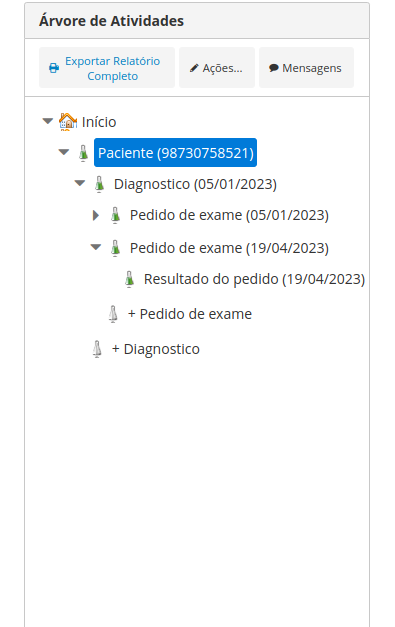
\includegraphics[width=0.8\textwidth]{imgs/Exemplo-Mestrado/arvore_medico.png}
        \caption{Visualização do workflow pela visão do médico, que não tem permissão de visualizar atividades de execução do pedido de exame.}
        \label{fig:arvore_medico}
    \end{subfigure}
    \hfill
    \begin{subfigure}[b]{0.45\textwidth}
        \centering
        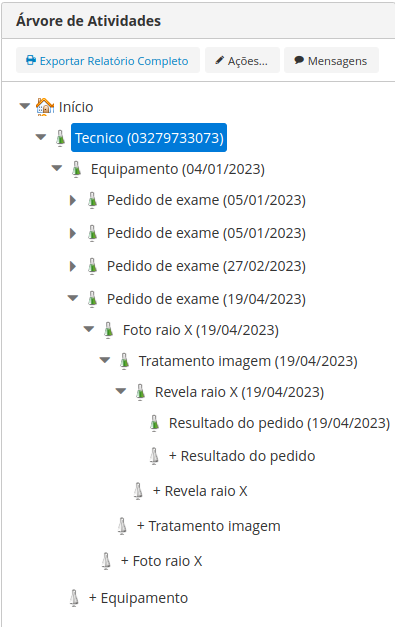
\includegraphics[width=0.75\textwidth]{imgs/Exemplo-Mestrado/arvore_tecnico.png}
        \caption{Visualização do workflow pela visão do técnico de laboratório, que executa as atividades do pedido de exame e executa também o resultado do pedido, disponibilizando para a visualização do médico.}
        \label{fig:arvore_tecnico}
    \end{subfigure}
    \caption{Demonstração de transições entre atividades dentro do Flux. Cada atividade executada é representada uma linha com a imagem de um frasco com líquido verde. Cada mudança de espaçamento entre as atividades mostra que existe transições entre a atividade sem a mudança de espaçamento e as com mudança de espaçamento.}
    \label{fig:arvore_medico_tecnico}

\end{figure}

Um exemplo disso é em um pedido de exame de sangue de um médico para um laboratório, que irá examinar a amostra e dar um resultado ao médico. Este médico só poderá continuar o processo de atendimento quando o técnico de laboratório tiver terminado de realizar todas as análises da amostra e executando uma atividade de resultado de análise, que o médico tem acesso, tendo assim a troca de informações entre médico e técnico de laboratório e melhorando a integração entre os dois processos.

% O que isso traz para os LIMS

A integração desta nova ferramenta a um LIMS melhora muito a eficiência e integração das atividades de um modelo de negócios com o outro, otimizando a troca de informações entre dois fluxos de trabalho. O médico pode receber uma notificação quando o exame ficar pronto, um técnico recebe notificação quando uma amostra chega e pode até ser feita a otimização deste caminho, com a amostra indo direto para uma máquina analisar.

Isso também facilita a utilização do software pelos usuários, já que fica mais intuitivo onde e quando o usuário deve entrar dentro da interface para acessar os dados que são de seu interesse.

% Porque isso é necessário?

\subsection{Usos}

É possível vincular atividades de diferentes BPMs umas as outras por meio do compartilhamento de atividades. Os BPMs que contém atividades compartilhadas devem ser modelados juntos para que toda a execução do fluxo de trabalho possa ser pensado e otimizado pensando em um processo colaborativo entre os usuários. Os usuários que irão utilizar o workflow poderão receber notificações sobre execuções de atividades compartilhadas por outros usuários e a modelagem também pode ser pensando para envio de notificações para que a execução possa ser feita de maneira mais efetiva. Um exemplo de utilização é a que um cientista pede a análise de uma amostra a um técnico de laboratório, que por sua vez recebe a notificação que o pedido foi feito, deixando disponíveis atividades para execução deste pedido. Quando concluída, o cientista recebe uma notificação de que a análise da amostra foi executada e que ele pode seguir com seu fluxo de trabalho.